\chapter{Evapotranspiration} \label{chap:et}
\renewcommand{\tabdir}{chapters/part_processes/evapotranspiration/tab}
\renewcommand{\figdir}{chapters/part_processes/evapotranspiration/fig}

\section{Introduction} \label{sec:et_intro}

This chapter describes approaches to model evapotranspiration. The focus is on very simple approaches relying on a two-step calculation procedure:
\begin{enumerate}
  \item Computation of a \emph{potential} evapotranspiration rate \etPot. This represents the maximum possible rate in the absence of water stress. It is basically limited by energy supply.
  \item Estimation of the \emph{actual} evapotranspiration rate \etReal{} from the potential rate taking into account the properties of vegetation and the limitation by a soil moisture deficit.
\end{enumerate}

%%%%%%%%%%%%%%%%%%%%%%%%%%%%%%%%%%%%%%%%%%%%%%%%%%%%%%%%%%%%%%%%%%%%%%%%%%%%%%%%
%%%%%%%%%%%%%%%%%%%%%%%%%%%%%%%%%%%%%%%%%%%%%%%%%%%%%%%%%%%%%%%%%%%%%%%%%%%%%%%%
%%%%%%%%%%%%%%%%%%%%%%%%%%%%%%%%%%%%%%%%%%%%%%%%%%%%%%%%%%%%%%%%%%%%%%%%%%%%%%%%

\section{Potential evapotranspiration} \label{sec:et:pot}

\section{Hargreaves model} \label{sec:et:pot:hargreaves}

This is a very simply model yielding estimates of \etPot{} with daily resolution. It requires as input
\begin{itemize}
  \item Incoming short-wave radiation
  \item Daily minimum and maximum temperature
\end{itemize}

If the radiation is given as a daily average value (instead of a sum), the Hargreaves model takes the form of \eqnref{eqn:et:pot:hargreaves}

\begin{align} \label{eqn:et:pot:hargreaves}
  \etPot = & CH \cdot \left( \frac{t_{max}+t_{min}}{2} + CT \right) \cdot \\
           & \sqrt{t_{max}-t_{min}} \cdot 0.0864 \cdot \radShortwaveIn{} \nonumber
\end{align}

with

\medskip
\begin{tabular}{p{0.25\columnwidth}p{0.55\columnwidth}}
  \etPot & Hargreaves potential evapotranspiration rate (mm/day) \\
  $t_{max}$, $t_{min}$ & Daily minimum and maximum of air temperature (\celsius) \\
  \radShortwaveIn{} & Daily average of incoming short-wave radiation (W/\sqm{}) \\
  0.0864 & Factor to convert \radShortwaveIn{} from W/\sqm{} into MJ/\sqm{}/day \\
  $CH$ & Empirical coefficient, $CH$= 0.0023 \\
  $CT$ & Empirical coefficient, $CT$= 17.8 \\
\end{tabular}


\section{Makkink model} \label{sec:et:pot:makkink}

The Makkink model is another simple approach to estimate potential evaporation using only temperature and downward short-wave radiation as predictors. The approach is discussed in detail by \citet{deBruin1987, Feddes1987, Hiemstra2011}.

Using convenient units, the basic equation without an additive empirical constant \citep[see][]{deBruin1987} is \eqnref{eqn:et:pot:makkink}

\begin{equation} \label{eqn:et:pot:makkink}
  \etPot = c \cdot \frac{s}{s + \gamma} \cdot \frac{\radShortwaveIn}{1000 \cdot \evapHeatWater \cdot \densityWater}
\end{equation}

with

\medskip
\begin{tabular}{lp{0.8\columnwidth}}
  \etPot & Makkink reference crop-evaporation (m/s) \\
  $s$ & Slope of the curve of saturation water vapor pressure (kPa / K) \\
  $\gamma$ & Psychrometric constant (kPa / K) \\
  $\radShortwaveIn$ & Incoming short-wave radiation (W/\sqm{}) \\
  $\evapHeatWater$ & Latent heat of water evaporation (kJ/kg) \\
  $\densityWater$ & Density of water ($\approx$ 1000 kg/\cbm{}) \\
  $1000$ & Factor to convert kJ into J \\
  $c$ & Dimensionless empirical constant, $c$=0.65 \\
\end{tabular}


The latent heat of water evaporation \evapHeatWater{} (kJ/kg) is simply a function of temperature (see \eqnref{eqn:evap_makkink_evapHeatWater} on page~\pageref{eqn:evap_makkink_evapHeatWater}). For the dimensionless term $s/(s + \gamma)$ \citet{Yao2009} present a convenient approximation based on the air temperature (see \eqnref{eqn:evap_makkink_dimlessFraction} on page~\pageref{eqn:evap_makkink_dimlessFraction}). A more accurate estimate is obtained, however, using the empirical expressions for $s$ and $\gamma$ (both in hPa/K) from \eqnref{eqn:slopeSatVapPress} and \eqnref{eqn:psychroConst}

\begin{align} 
  s=& 6.11 \cdot exp\left(\frac{17.3 \cdot \airtemp}{237.3 + \airtemp} \right) \cdot \label{eqn:slopeSatVapPress} \\
    & \frac{4105.3}{(237.3 + \airtemp)^2} \nonumber \\
  \gamma=& 0.016286 \cdot \frac{\airPressure}{\evapHeatWater(\airtemp)} \label{eqn:psychroConst}
\end{align}

where \airPressure{} is the air pressure (hPa) and \airtemp{} is the air temperature  in \celsius{} \citep{Dyck1995}.

%%%%%%%%%%%%%%%%%%%%%%%%%%%%%%%%%%%%%%%%%%%%%%%%%%%%%%%%%%%%%%%%%%%%%%%%%%%%%%%%
%%%%%%%%%%%%%%%%%%%%%%%%%%%%%%%%%%%%%%%%%%%%%%%%%%%%%%%%%%%%%%%%%%%%%%%%%%%%%%%%
%%%%%%%%%%%%%%%%%%%%%%%%%%%%%%%%%%%%%%%%%%%%%%%%%%%%%%%%%%%%%%%%%%%%%%%%%%%%%%%%

\section{Real evapotranspiration} \label{sec:et:real}

In the approaches described here, the rate of real evapotranspiration \etReal{} is computed by multiplying the potential rate \etPot{} with dimensionless correction factors. Typically, these factors account for
\begin{itemize}
  \item the different transpiration characteristics of the actual vegetation as compared to the reference vegetation to which \etPot{} refers (usually short grass). These factors are known as \emph{crop factors} (\secref{sec:et:real:cropfactors}).
  \item the reduction of plant transpiration due to soil moisture limitation (\secref{sec:et:real:soilmoisture}).
\end{itemize}

\subsection{Crop factors} \label{sec:et:real:cropfactors}

For some equations to estimate \etPot{}, an extensive set of crop factors has been established based on empirical research. The values vary between different crops and also account for the different stages of plant grow, \ie{} seasonality. For the Makkink model (\secref{sec:et:pot:makkink}), crop factors can be found in \citet{Feddes1987}. For wider applicability, it is desireable to derive the crop factors from other easily available data. A potential candidate is the leaf-area index \leafAreaIndex. Based on figure \figref{fig:et:real:cropfactor-LAI}, an approximate relation between the crop factor of the Makkink model and the \leafAreaIndex{} can be derived (\eqnref{eqn:et:real:cropfactor-LAI}).

\begin{equation} \label{eqn:et:real:cropfactor-LAI}
  \text{crop factor} \approx 0.14 \cdot \leafAreaIndex + 0.4 
\end{equation}

Note that, following the conventional definition of \etPot{}, the crop factor should take a value of one for the reference crop (typically actively growing gras of 12~cm height with unlimited water supply). Assuming that the corresponding \leafAreaIndex{} is about 5 \citep[see, \eg][]{Misra1981} or \citep[][page 11]{Bremicker2006}, the simplest linear approach would be \eqnref{eqn:et:real:cropfactor-LAI-simple}.

\begin{equation} \label{eqn:et:real:cropfactor-LAI-simple}
  \text{crop factor} \approx 0.2 \cdot \leafAreaIndex
\end{equation}

This equation, however, implies that evapotranspiration from bare soil is zero. In reality, a non-zero intercept is more plausible.

During calibration of a hydrological model for the Upper Neckar Basin (Germany), the relation shown in \eqnref{eqn:et:real:cropfactor-LAI-Neckar} was identified. It yielded the best result for a larger part of the catchment (gage Kirchtellinsfurt, 2300~\sqkm). The optimum parameters for smaller sub-basins were similar. The assumed \leafAreaIndex{} of grassland vegetation in that model was 5.

\begin{equation} \label{eqn:et:real:cropfactor-LAI-Neckar}
  \text{crop factor} \approx 0.16 \cdot \leafAreaIndex + 0.2 
\end{equation}



\begin{figure}
  \centering
  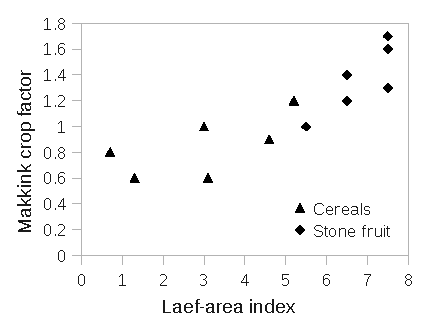
\includegraphics[width=0.75\columnwidth]{\figdir/cropfactor_LAI.eps}
  \caption[Relation between the crop factor (for Makkink model) and the leaf-area index (\sqm/\sqm) for two selected crops.]{Relation between the crop factor (for Makkink model) and the leaf-area index (\sqm/\sqm) for two selected crops. Crop factors and the corresponding values of \leafAreaIndex{} were taken from \citet{Feddes1987} and \citet{Ludwig2006}, respectively. \label{fig:et:real:cropfactor-LAI}}
\end{figure}

\subsection{Influence of soil moisture} \label{sec:et:real:soilmoisture}

A widely used scheme to account for the limitation of real evapotranspiration by soil moisture is illustrated in \figref{fig:et:real:soilmoisture}. This approach uses two empirical constants $rs_{et min}$ and $rs_{et max}$ representing threshold values of relative soil saturation. For very dry soil with relative saturation between 0 and $rs_{et min}$, real evapotranspiration is zero. For wet conditions with relative saturation between $rs_{et max}$ and 1, the rate of real evapotranspiration \etReal{} is equal to the potential rate \etPot{}. For intermediate conditions, \etReal{} is assumed to vary linearily with soil saturation (\ie{} soil moisture). Mathematically, this is expressed by \eqnref{eqn:et:real:soilmoisture}.

\begin{equation} \label{eqn:et:real:soilmoisture}
  \frac{\etReal}{\etPot} = min\left(1, max\left(0, \frac{rs-rs_{et min}}{rs_{et max}-rs_{et min}} \right)\right)
\end{equation}

\begin{figure}
  \centering
  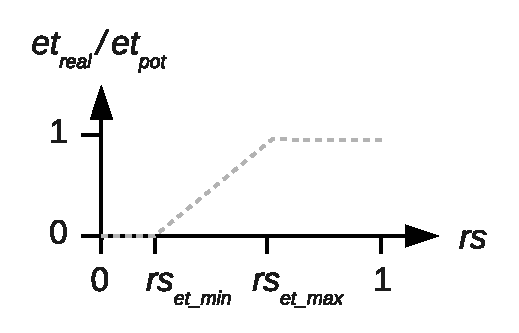
\includegraphics[width=0.6\columnwidth]{\figdir/soilMoistureEffect.eps}
  \caption{Ratio of real to potential evapotranspiration \etReal/\etPot{} as a function of relative soil saturation $rs$. \label{fig:et:real:soilmoisture}}
\end{figure}

In this definition, the relative soil saturation $rs$ is the quotient of the current soil water content $\soilWaterContent$ and the soil-specific maximum value $\soilWaterContentMax$. Thus, the two parameters $rs_{et min}$ and $rs_{et max}$ take values in range 0 to 1. A reasonable estimate for $rs_{et min}$ can be obtained from data on the water content at the wilting point. This value varies considerably between soil types as illustrated in \figref{fig:et:real:pFCurve}.

\begin{figure}
  \centering
  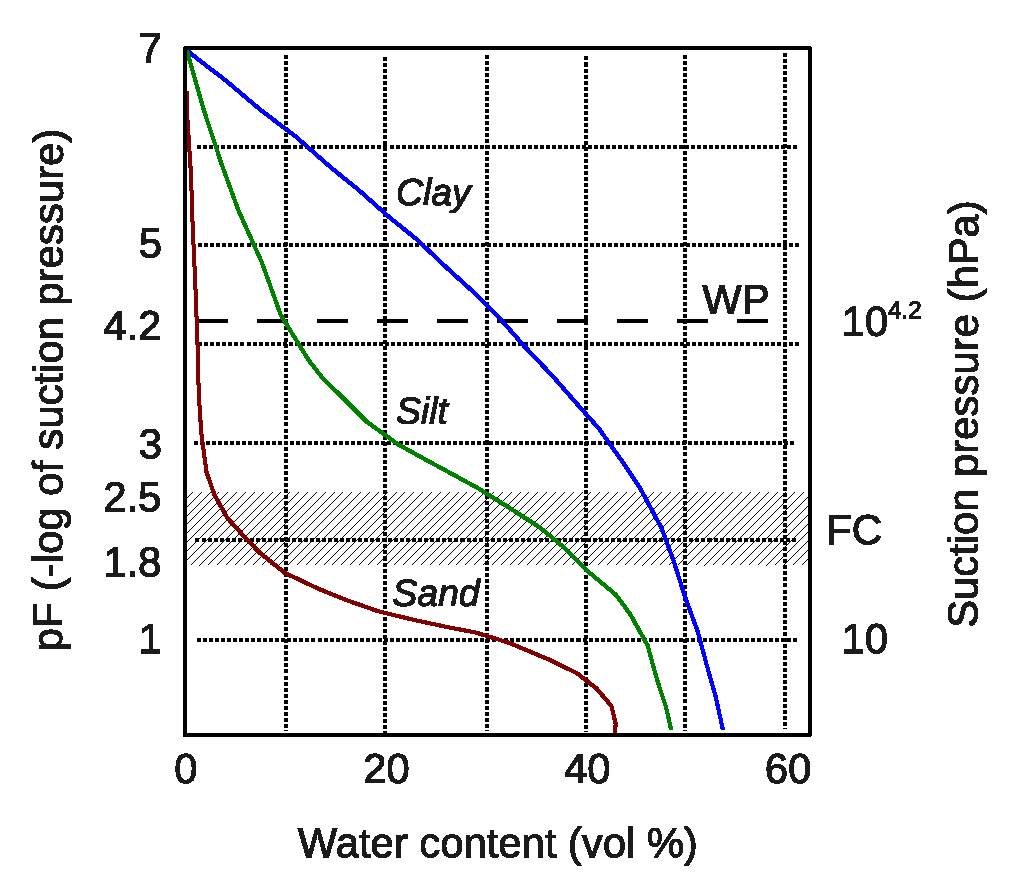
\includegraphics[width=0.9\columnwidth]{\figdir/pF_and_waterContent.eps}
  \caption{Typical relation between water content and suction pressure for different soil types. The permanent wilting point is defined as pF=4.2 ($\approx$ 1500 kPa). The hatching marks the typical range of the field capacity found in soils. Adapted from \citet{Scheffer1998}. \label{fig:et:real:pFCurve}}
\end{figure}

Some characteristic values of soil water content (based on \figref{fig:et:real:pFCurve}) and the corresponding estimates of model parameters are presented in \tabref{tab:et:real:soilmoisture}.

\begin{table}
  \caption{Characteristic values of the soil water content $\soilWaterContent$ and corresponding estimates of model parameters derived from \figref{fig:et:real:pFCurve}. \label{tab:et:real:soilmoisture}}
  {\small
  \begin{tabular}{|rlllll|} \hline
    \rowcolor[gray]{0.9}
         &                        & $\soilWaterContent$ at & $\soilWaterContent$ at & & \\
    \rowcolor[gray]{0.9}
    Soil & $\soilWaterContentMax$ & pF=2.5 & pF=4.2 & $rs_{et max}$ & $rs_{et min}$ \\ \hline
    Sand & 0.43 & 0.03 & 0.02 & < 0.07 & 0.05 \\
    Silt & 0.48 & 0.3  & 0.1  & < 0.63 & 0.21 \\
    Clay & 0.53 & 0.46 & 0.32 & < 0.86 & 0.6 \\
  \hline
  \end{tabular} 
  }
\end{table}
